\documentclass[10pt]{beamer}

\usetheme{Warsaw}
\beamertemplatenavigationsymbolsempty

\usepackage[utf8x]{inputenc}
\usepackage[francais]{babel}
\usepackage{hyperref}
\usepackage{amsmath}
\usepackage{graphicx}
\usepackage{tikz}
\usepackage{multicol}
\usetikzlibrary{automata,positioning}
\graphicspath{{./img/}}
\DeclareGraphicsExtensions{.png, .jpeg, .jpg}


\renewcommand*\thesection{\arabic{section}}


\AtBeginSection[]{%
  \begin{frame}<beamer>
    \frametitle{Plan}
    \tableofcontents[sectionstyle=show/hide,subsectionstyle=hide/show/hide]
  \end{frame}
  \addtocounter{framenumber}{-1}
}

\setbeamertemplate{footline}[frame number]


\title{Statistical Machine Translation for Query Expansion in Answer
  Retrieval\\ 
\small
Stefan Riezler, Alexander Vasserman, Ioannis Tsochantaridis, Vibhu
Mittal and Yi Liu}

\author{Rémi Bois, Agathe Mollé}
\date{\today}

\begin{document}

\begin{frame}
  \maketitle
  \vfill
  \begin{figure}
    
\includegraphics[width=0.20\textwidth]{logo_univ_nantes}
  \end{figure}

\end{frame}

\begin{frame}
  \tableofcontents
\end{frame}

\section{Introduction}
\label{sec:intro}


\section{Question Answering}
\label{sec:QA}

\begin{frame}
  \frametitle{Répondre à des questions}
  % questions en langage naturel, réponses en langage naturel
  \begin{block}{Format}
    Les questions sont posées en langage naturel.

    Exemple : How to live with cat allergies ?

    Les réponses sont également données en langage naturel.
  \end{block}
\end{frame}

\begin{frame}
  \frametitle{Une tâche de Recherche d'Informations}
  % recherche dans un ensemble de FAQ

  \begin{block}{Comment répondre ?}
    On ramène la tâche de question/réponse à une recherche dans une
    base de FAQ. 

    Les documents retournés sont les réponses des
    questions d'une FAQ.
  \end{block}
\end{frame}

\section{Ajout de la paraphrase et de la traduction de questions}
\label{sec:paratrans}

\begin{frame}
  \frametitle{Paraphraser pour améliorer la précision}
  % présenter l'intuition et un exemple
\end{frame}

\begin{frame}
  \frametitle{Comment paraphraser ?}
  % double traduction
\end{frame}

\begin{frame}
  \frametitle{Sélection des paraphrases}
  %formule
\end{frame}

\begin{frame}
  \frametitle{La traduction automatique pour améliorer les résultats
    ?}
  % traduction question -> réponse + exemple
\end{frame}

\section{Corpus et données d'entraînement}
\label{sec:corpus}

\begin{frame}
  \frametitle{L'entraînement du module de paraphrase}
  % russe truc
\end{frame}

\begin{frame}
  \frametitle{Le corpus composé de FAQ}
  % présentation du corpus, stats etc...
  
\end{frame}


\section{Résultats}
\label{sec:results}


\begin{frame}
  \frametitle{Les données de test}
  \begin{block}{Données}
    20 réponses évaluées pour chacune des 60 questions posées.
  \end{block}

  \pause

  \begin{block}{Evaluation}
    2 juges, avec discussion lors d'un désaccord.
    
    Jugement en 3 critères :
    \begin{description}
    \item[adéquat] La réponse est contenue dans le document retourné
    \item[matériel] Pas de réponse exacte mais des informations importantes
    \item[insatisfaisant] Le besoin d'information de l'utilisateur
      n'est pas satisfait.
    \end{description}
  \end{block}
\end{frame}

\begin{frame}
  \frametitle{Baseline}

  \begin{block}{Mesure tfidf}
    La requête est lancée et les résultats retournés sont calculés
    avec une mesure tfidf classique.
  \end{block}
  \pause

  \begin{block}{Local expansion}
    Correspond à une extension de requête locale classique :

    \begin{itemize}
    \item La requête est lancée une première fois
    \item Les termes les plus importants (tfidf) des premiers
      documents retournés sont ajoutés à la requête
    \item La requête est relancée avec les termes originaux et les
      nouveaux termes
    \end{itemize}
  \end{block}
  % description de la baseline
  % description du S_2@n
\end{frame}

\begin{frame}
  \frametitle{Les détails du tfidf utilisés}

  \begin{block}{Vecteur de poids}
    \begin{figure}[h]
      \centering
      $<0.0, 1.0, 0.0, 0.0, 0.5, 0.5, 0.2, 0.3>$
    \end{figure}
    
    
    Les poids du vecteurs correspondent à :

    \begin{enumerate}
    \item Le texte de tout le document
    \item Le texte de la question
    \item Le texte de la réponse
    \item Le texte du titre
    \item Chacun des textes ci-dessus, sans les stopwords
    \end{enumerate}

    Le but du second poids est de prendre en compte les termes
    interrogatifs (when, where, which, ...)

  \end{block}
  \pause
  \begin{block}{La mesure utilisée}
    Comparaison des vecteurs via la mesure Cosine
  \end{block}

\end{frame}

\begin{frame}
  \frametitle{Résultats}
  % le tableau
  \begin{figure}[h]
    \centering
    \begin{tabular}[h]{|c|c|c|c|c|}
    \hline
    & $S_2@10$ & $S_2@20$ & $S_{1,2}@10$ & $S_{1,2}@20$\\
    \hline
    baseline tfidf & 27 & 35 & 58 & 65\\
    local expansion & 30 (+11.1) & 40 (+14.2) & 57 (-1) & 63 (-3)\\
    SMT-based expansion & 38 (+40.7) & 43 (+22.8) & 58 & 65\\
    \hline
  \end{tabular}

    \caption{Résultats}
    \label{fig:res}
  \end{figure}

\end{frame}

\begin{frame}
  \frametitle{Explication des résultats}

  \begin{figure}[h]
    \centering
    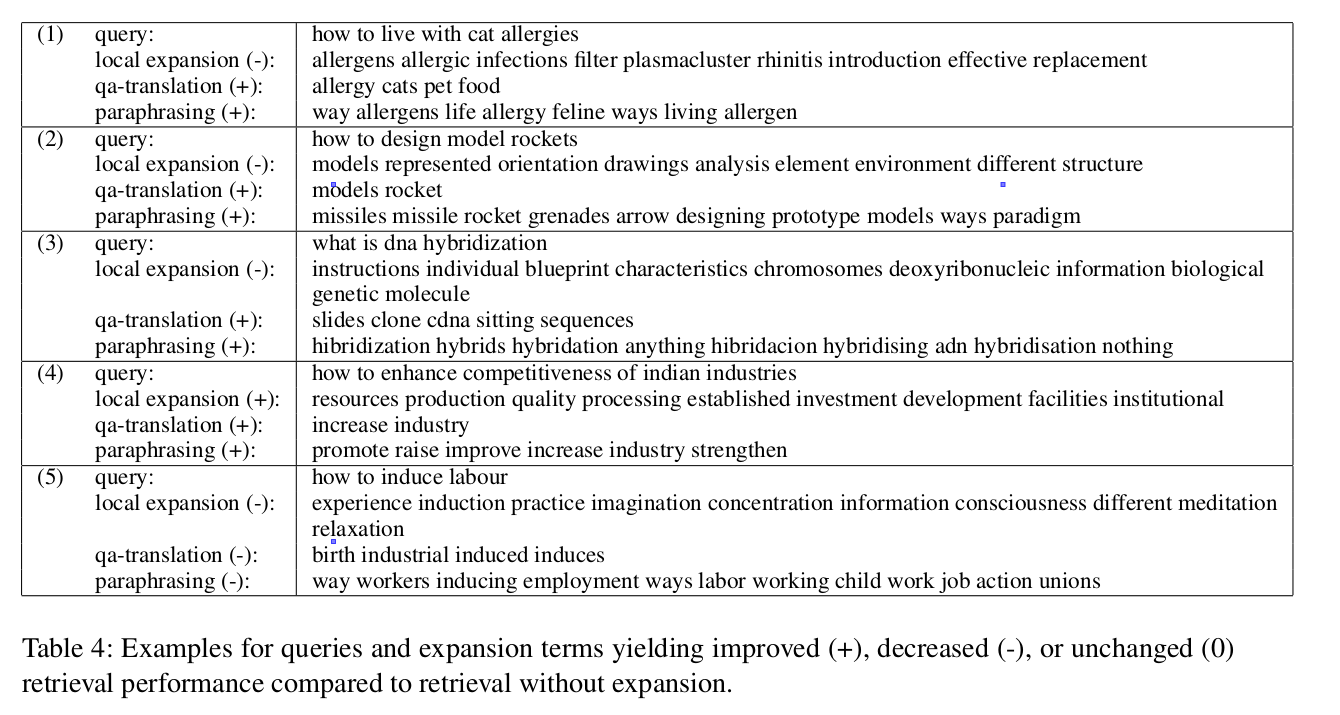
\includegraphics[width=\textwidth]{table4}
    \label{fig:res}
  \end{figure}
  % tableau 4 de l'article
\end{frame}

\section{Conclusion}
\label{sec:conclusion}


\begin{frame}
  \frametitle{Une méthode efficace}
  % approche nouvelle (?)
\end{frame}

\begin{frame}
  \frametitle{Quelques limites}
  Il semble que beaucoup de termes retrouvés par la méthode de
  paraphrase et de traduction correspondent en fait à des variations
  du même terme (eg. allergens, allergy, allergies, ...). Un stemming
  aurait permit de lever ces ambiguïtés sans avoir à recourir à ce système.
  % stemming ? taille du corpus de test ?
\end{frame}


\end{document}